\chapter{Task}
\label{task}
A task implementation is very specific for each plattform.

The language report indicates the task state diagram from 
fig. \ref{taskStatesPEARL90}. There is not difference made between {\em running} and {\em runable}. The switching between these two states is done by the
operating system automatically --- not visible to the PEARL application.

\begin{figure}[bpht]
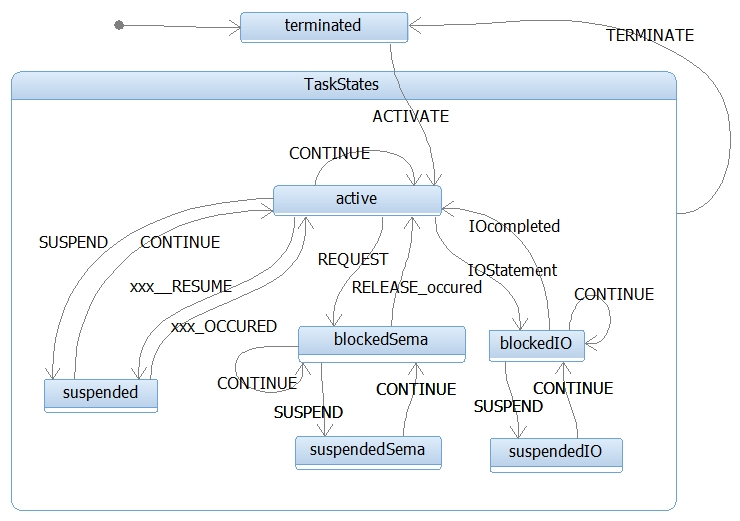
\includegraphics[width=14cm]{taskStatesPEARL90.jpg}
\caption{Task statediagram derived from the language report.
The transition \texttt{XXX\_RESUME} and \texttt{XXX\_OCCURED} denote 
the possiblities AFTER/AT/WHEN and the corresponding events.}
\label{taskStatesPEARL90}
\end{figure}

To trigger the events in the state diagram suitable methods in the task 
objects are provided. 

RTOS-UH used a different model, where termination while an active i/o statement
is delayed until the next end-of-record. 
This behavior is reasonable and is applied for termination and
suspending a task. The new state diagram is shown in 
fig. \ref{taskStatesOpenPEARL}.
The transitions from the  states {\em terminatePending} and 
{\em suspendPending}  are triggered from the i/o-system when a end-of-record
({\em SKIP}) is encountered or the i/o-statement becomes completed.

\begin{figure}[bpht]
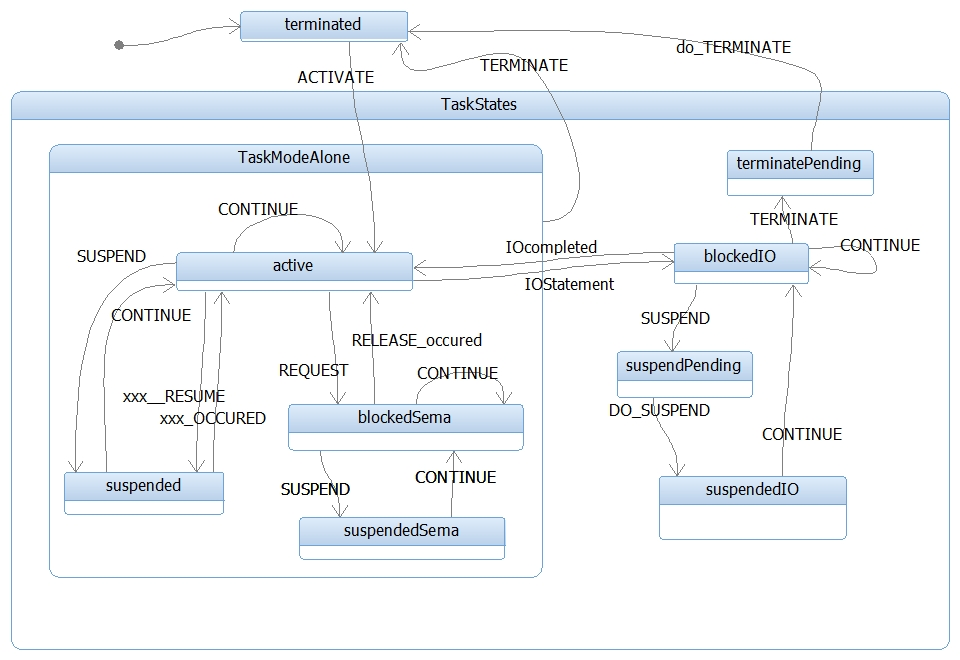
\includegraphics[width=14cm]{taskStatesOpenPEARL.jpg}
\caption{Task statediagram in OpenPEARL.
The transition \texttt{XXX\_RESUME} and \texttt{XXX\_OCCURED} denote 
the possiblities AFTER/AT/WHEN and the corresponding events.}
\label{taskStatesOpenPEARL}
\end{figure}

Several classes support the tasking operations:
\begin{description}
\item[class Interrupt] provides the semantics of the PEARL language interrupts
\item[class Semaphore] provides PEARL semaphore semantics with simultanous
   locking on semaphore arrays.
\item[class TaskTimerCommon] provides an interface for the plattform
   specific class \verb|TaskTimer|. 
\item[class TaskCommon] provides most of the error checking depending on
   the task state and tasking operation, as well as plattform independent
   parts of the tasking operations. Theses operations delegate the concrete
   plattform specific operation to the plattform specific implementation
   in the class \verb|Task|. The api methods in TaskCommon perform some
    parameter checks and look the mutex for all tasks before delegating 
    the job to the plattform specific implementation. 
    The mutex must be unlocked by the target specific implementation 
    after completion of the job. Some operation may need to release and 
    rerequest the mutex in the target specific job --- e.g. suspend,
    which has to block the task until it is continued by another task
    or a scheduded continue.

\item[class TaskList] provides a list of all defined PEARL tasks
\item[class TaskMonitor] keeps track of all scheduled and active tasks and
   detects the end of the application.
\item[class Control] allows setting the exit status for the application. 
  The treatment of this status is plattform specific.
\end{description}

\section{Thread Safety}
The task state is stored in the task control block, which is realized
by attributes of the \verb|Task|-objects.
The mutual exclusion is realized by  public class methods
\begin{itemize}
\item \verb|TaskCommon::mutexLock()|
\item \verb|TaskCommon::mutexUnlock()|
\end{itemize}
 
This mutex is used in the task related classes, as well as in the interrupt
and semphore related classes. 

All tasking related methods, which check or modify  the tasks state lock the 
mutex variable. Some parts of execution are delegated to plattform specific
code. For details about unlocking the mutex please check the code
documentation from doxygen.



\section{Specification and Declaration}
\begin{description}
\item[SPCTASK] makes the forward declararion of the task object.
    The compiler must add the forward declaraction of all tasks
    used in the module before the first declaration, since C++
    variables have a scope from the line of declaration until 
    the end of the block, which contains the declaration.
    The macro has the tasks name as parameter.
\item[DCLTASK] defines the task itself. The DCLTASK macro is followed
    by a block of statements, which define the tasks content.
    The macro has the tasks name, priority and main-attribute as
    parameter. 
    Priority and isMain-attribute are wrapped by the compiler 
    into \verb|Prio|- and \verb|BitString<1>|-type.
\end{description}

The implementation of task handling is plattform specific.
Each plattform specific implementation need:
\begin{enumerate}
\item  a class {\em Task} which is derived from {\em TaskCommon}.
\item the suitable definition of the \verb|DCLTASK|- and \verb|SPCTASK|-macros
\item the implementation of the tasking methods
\item a mechanism which activates on system start
   all defined tasks containing the isMain-attribute with true. 
   The sequence is defined by the tasks priority. 
   No priority corresponds to the weakest priority.
\item a mechanism which enables a default signal handler for each task
\item a mechanism which enshures the task termination at the end of
   the task body
\end{enumerate}

\paragraph{Notes}\ \\
\begin{itemize}
\item The macros SPCTASK and DCLTASK are currently sufficient only for
    PEARL programs with one module. When multi-module programs
    are supported by the compiler, the GLOBAL-attribute should be 
    passed additionally to both macros.
\end{itemize}

\section{me-Pointer}
The DCLTASK-macro must define an object with the name of the
task with the type {\em Task}.
The macro must enshure that a variable  {\em Task * me;} exists
and points to the tasks object. This pointer is used
by the compiler to trigger tasking operations of the current
task.

This pointer is passed to every procedure as hidden (first) parameter.
By this mean, each procedure may do tasking operations upon the
task, which uses the procedure.
The {\em me}-pointer is defined to be from the base class  {\em TaskCommon}. 
The runtime tasks are derived from this class, so the pointer to the current 
task fits to {\em me}.

\section{Task Priority}
The tasks default priority is defined in the TASK-statement and passed
as second parameter in the DCLTASK-macro.
Scheduling calls may alter the tasks priority. This new priority is valid 
until a new priority is assigne. At restart of the task the default 
priority is used again. Each plattform must provide a class \verb|PrioMapper|.

If the concrete target system (like linux) does not support 255 
 application priorities, the method \verb|freomPearl()| must throw
an exception.

\section{Tasking Methods (class TaskCommon)}
For Task objects there are methods defined to do the tasking actions like
ACTIVATE, TERMINATE, SUSPEND, CONTINUE , RESUME and PREVENT.

Scheduled operations are possible in combination of ACTIVATE, 
CONTINUE and RESUME.
The schedule (like AT, ALL, AFTER, WHEN,..) is passed to the 
tasks methods. The way of treatment (by timers, specific timer threads, ... )
is decided by the plattform code.
The parameter {\em condition} of the methods for ACTIVATE, CONTINUE and RESUME
codes bit by bit, which additional parameters are really used.
The enumeration {\em TaskScheduling} defines the constants:
Only marked parameters are treated by the runtime system.
Illegal combinations are rejected by an exception.
\begin{CppCode}
      enum TaskScheduling {
         AT = 1, AFTER = 2, WHEN = 4, ALL = 8,
         DURING = 16, UNTIL = 32, PRIO = 64
      };
\end{CppCode}

The API of tasks is defined in {\em TaskCommon}.

The default parameters enshure proper values, in case the compiler omits 
parameters, which are not required for the current runtime system call.
Omitting parameters has no effect on the execution speed.
The default parameters are useful when using the runtime system
directly from C++ for e.g. testing purpose.

\subsection{Task Activation}
The task activation may be done immediatelly or scheduled. 
In case of immediate activation the task must be in {\em terminated} state or
a signal is induced.
In case of scheduled activation - only the last scheduled activation job is
valid. If the task is not terminated when the schedule condition becomes valid,
the scheduled operation is ignored this time.

A \verb|WHEN|-condition requires to pass the pointer to the interrupt source
as last parameter. Due to the up-cast in the interrupt specification, this
is just the user supplied identifier at this point.

\begin{CppCode}
void activate(TaskCommon* me,
              int condition = 0,
              Prio prio = Prio(),
              Clock at = Clock(),
              Duration after = Duration(),
              Duration all = Duration(),
              Clock until = Clock(),
              Duration during = Duration(),
              Interrupt *when = 0);
\end{CppCode}

This method delegates the concrete tasks activation to the method
\verb|directActivate(...)|, which must be provided in the plattform specific
part.

\subsection{Task termination}
The task termination may be called from the task self, or from another task.
The task shall terminate immediatelly. In case an I/O-operation is in progress
the task termination is delay until a suitable point is reached
(e.g. end-of-record).

\begin{CppCode}
virtual void terminate(TaskCommon* me) = 0;
\end{CppCode}

This method delegates the concrete tasks termination to the methods
\verb|terminateMySelf(...)| and \verb|terminateFromOtherTask()|,
which must be provided in the plattform specific part.

\subsection{Task Suspending}
A task may suspend itself or suspend another task.
The task to be suspended must be in running state. If the task state
is different, a signal is induced.
The suspend call shall 
stop the execution of the task immediatelly with the possiblity to 
continue later.
In case an I/O-operation is in progress the task suspending is delayed
until a suitable point is reached (e.g. end-of-record),. 
If the task is blocked on e.g. a semaphore it does no longer try to get 
the semaphore.
 
\begin{CppCode}
void suspend(TaskCommon* me);
\end{CppCode}

This method delegates the concrete tasks suspend operation to the methods
\verb|suspendMySelf(...)| and \verb|suspendFromOtherTask()|,
which must be provided in the plattform specific part.

\subsection{Task Continuation}
A task may be continued if it is running or suspended.
Since \verb|continue| is a revered key word, the method is named \verb|cont|.

A \verb|WHEN|-condition requires to pass the pointer to the interrupt source
as last parameter. Due to the up-cast in the interrupt specification, this
is just the user supplied identifier at this point.

\begin{CppCode}
void cont(TaskCommon* me,
          int condition = 0,
          Prio prio = Prio(),
          Clock at = Clock(),
          Duration after = Duration(),
          Duration all = Duration(),
          Clock until = Clock(),
          Duration during = Duration(),
          Interrupt *when = 0) = 0;
\end{CppCode}

This method delegates the concrete tasks continuation to the methods
\verb|continueSuspended(...)| and \verb|continueFromOtherTask()|,
which must be provided in the plattform specific part.

\subsection{Task Delay}
The execution of a task may be suspended for a while.
Only one value from {\em at}, {\em after} and {\em when} may be selected
in the condition field. 


\begin{CppCode}
void resume( int condition = 0,
             Clock at = Clock(),
             Duration after = Duration(),
             Interrupt * when = 0);
\end{CppCode}
This method delegates the concrete tasks continuation to the method
\verb|resume2(...)|,
which must be provided in the plattform specific part.


\subsection{Delete Task Schedules}
To remove scheduled operations for a task the method {\em prevent} is supplied.

\begin{CppCode}
void prevent(TaskCommon* me);
\end{CppCode}

\section{Example}
\begin{PEARLCode}
T1: TASK PRIO 10;
   SUSPEND;
END;

T2: TASK MAIN;
   AFTER 5 SEC ALL 1 SEC ACTIVATE T1;
   AFTER 7 SEC RESUME;
   CONTINUE T1;
   PREVENT T1;
   
END;
\end{PEARLCode}

\begin{CppCode}
SPCTASK(T1);
SPCTASK(T2);

DCLTASK(T1, Prio(Fixed<15>(10)), BitString<1>(0)) {
  me->suspend(me);
}

DCLTASK(T2, Prio(255), BitString<1>(1)) {
  Fixed<31> y;

  T1.activate(me,
              Task::AFTER | Task::ALL,
              Prio(),
              Clock(),
              Duration(5.0),
              Duration(1.0) );
  me->resume(Task::AFTER, Duration(7.0) );
  T1.cont(me);
  T1.prevent(me);
}

\end{CppCode}

\section{Error Tracing}
The error handling of PEARL is done with SIGNALs.
They are very similar to the exceptions in C++ and JAVA. 
The run time systems throws exepctions which are organized in a
hierarchy to catch several exceptions of one kind in one step.
To provide a backtrace to the originating PEARL source line, the compiler 
must add tracing functions.
\begin{CppCode}
Task::setSource(const char * fileName, int lineNumber);
\end{CppCode}
The method {\em setSource()} is supplied with the valiues from
the PEARL source file.

\begin{CppCode}
const char* filename =  "api.prl";
SPCTASK(t1);
SPCTASK(t2);

DCLTASK(t1,10,1) {
   me->setLocation(10,filename);
   pearlrt::Duration d(5.0);
   me->setLocation(11,filename);
   pearlrt::Duration dur;
   me->setLocation(12,filename);
   dur = d*10.0;
   me->setLocation(13,filename);
   printf("5 sec delay\n");
   me->setLocation(14,filename);
   me->resume(pearlrt::Task::AFTER, pearlrt::Clock(),d);
   me->setLocation(15,filename);    
   printf("after 5 sec all 2 sec during 30 sec activate  t2\n");
   printf("    -> 16 activations\n");
   me->setLocation(16,filename);
   t2.activate(me, pearlrt::Prio(30),
               pearlrt::Task::AFTER|pearlrt::Task::DURING|pearlrt::Task::ALL,
               pearlrt::Clock(), d, pearlrt::Duration(2.0), // at, all
               pearlrt::Clock(),d*6.0,0) ;    
}

int t2counter=0;
DCLTASK(t2,20,0) {
   me->setLocation(17,filename);
   printf("t2 started (%d)\n", ++t2counter);
   me->setLocation(18,filename);
   pearlrt::Duration d(10.0);
   me->setLocation(19,filename);
   d = d / (t2counter-2);
}
\end{CppCode}

As result, uncaught SIGNALS would produce an error message like:
\begin{verbatim}
***************************
* Signal "fixed overflow" occured in api.prl at line 19
* Task T2 terminated
***************************
\end{verbatim}

Details about signal-handling is described in the section about signals.

